%% =============================================================================
%% main.tex
%% A Kirkpatrick-based Framework for Integrating Safety and Sustainability in
%% Aviation Maintenance: A Case Study on Waste Reduction and Resource Efficiency
%%
%% Target journal: Journal of Air Transport Management (Elsevier)
%% Template: Elsevier CAS (cas-dc, double column)
%% =============================================================================

\documentclass[a4paper,fleqn,oneside]{cas-dc}

% Tipografia ----------------------------------------------------------------
% Estratégia: lmodern para texto (ligaduras fi/ff/fl em todos os tamanhos);
% cas-dc.cls continua provendo STIX para math via seu próprio setup.
% A combinação reescreve os defaults de família de texto sem tocar no math.
\usepackage[utf8]{inputenc}
\usepackage[T1]{fontenc}
\renewcommand{\rmdefault}{lmr}
\renewcommand{\sfdefault}{lmss}
\renewcommand{\ttdefault}{lmtt}
\usepackage[expansion=false]{microtype}

% Bibliografia ---------------------------------------------------------------
\usepackage[authoryear,longnamesfirst]{natbib}

% Float placement -- figuras e tabelas movidas manualmente para o final do
% documento (depois da bibliografia). Cada float usa [!tbp] como placement
% para evitar páginas brancas intermediárias.

% Gráficos e diagramas ------------------------------------------------------
\usepackage{tikz}
\usetikzlibrary{
  positioning,
  arrows.meta,
  shapes.geometric,
  shapes.misc,
  calc,
  fit,
  backgrounds,
  patterns
}
\usepackage{pgfplots}
\pgfplotsset{compat=1.18}
\usepgfplotslibrary{groupplots}

% Tabelas adicionais --------------------------------------------------------
\usepackage{tabularx}
\usepackage{array}

% Lista customizável (leftmargin etc.) -------------------------------------
\usepackage{enumitem}

% Cores (paleta acessível, Elsevier-friendly) -------------------------------
\definecolor{kpBlue}{HTML}{2171B5}
\definecolor{kpBlueL}{HTML}{C6DBEF}
\definecolor{kpGreen}{HTML}{2C9F2C}
\definecolor{kpGreenL}{HTML}{CDEFCD}
\definecolor{kpOrange}{HTML}{E69138}
\definecolor{kpOrangeL}{HTML}{FCE5CD}
\definecolor{kpRed}{HTML}{CC0000}
\definecolor{kpRedL}{HTML}{F4CCCC}

% Hyperref ------------------------------------------------------------------
\hypersetup{
  colorlinks=true,
  linkcolor=kpBlue,
  citecolor=kpBlue,
  urlcolor=kpBlue
}

% Macros úteis (acronyms as plain text macros) ------------------------------
\usepackage{xspace}
\newcommand{\AS}{AS9100\xspace}
\newcommand{\ICAO}{ICAO\xspace}
\newcommand{\FAA}{FAA\xspace}
\newcommand{\EASA}{EASA\xspace}
\newcommand{\ANAC}{ANAC\xspace}
\newcommand{\IATA}{IATA\xspace}
\newcommand{\SAE}{SAE\xspace}
\newcommand{\SMS}{SMS\xspace}
\newcommand{\MRO}{MRO\xspace}
\newcommand{\ERP}{ERP\xspace}
\newcommand{\LMS}{LMS\xspace}
\newcommand{\CAR}{CAR\xspace}
\newcommand{\CAA}{CAA\xspace}
\newcommand{\ROI}{ROI\xspace}
\newcommand{\NPV}{NPV\xspace}
\newcommand{\ESG}{ESG\xspace}
\newcommand{\CoQ}{CoQ\xspace}

\begin{document}

% =============================================================================
% FRONTMATTER
% =============================================================================

\title[mode=title]{A Kirkpatrick-based Framework for Integrating Safety and Sustainability in Aviation Maintenance: A Case Study on Waste Reduction and Resource Efficiency}

\shorttitle{Kirkpatrick framework for safety \& sustainability in MRO}
\shortauthors{Pereira and Gon\c{c}alves}

% Autores -------------------------------------------------------------------
\author[1,2]{Jos\'e Cristiano Pereira}[
  prefix=Dr.,
  role=Researcher,
  orcid=0000-0002-2329-0560
]
\cormark[1]
\ead{josecristiano.pereira@ucp.br}
\credit{Conceptualization, Methodology, Investigation, Formal analysis,
        Writing -- original draft, Supervision, Funding acquisition,
        Project administration}

\author[1]{Heitor Oliveira Gon\c{c}alves}[
  orcid=0000-0002-5866-2213
]
\ead{heitorhog@gmail.com}
\credit{Data curation, Visualization, Validation,
        Writing -- review \& editing}

% Afiliações ----------------------------------------------------------------
\affiliation[1]{
  organization={Departamento de Engenharia e Computa\c{c}\~ao,
                Universidade Cat\'olica de Petr\'opolis (UCP)},
  city={Petr\'opolis},
  state={RJ},
  country={Brazil}
}

\affiliation[2]{
  organization={GE Aviation},
  country={Brazil}
}

\cortext[1]{Corresponding author.}

% =============================================================================
% ABSTRACT (rewritten per Reviewer comment #7: economic outcomes upfront)
% =============================================================================
\begin{abstract}
Within high-risk industries such as aviation maintenance, safety and
sustainability are intrinsically linked: maintenance errors not only drive
accidents but also generate substantial resource waste through rework, scrap
and the loss of human capital. This case study operationalises the Kirkpatrick
four-level model (Reaction, Learning, Behaviour, Results) over a twelve-month
intervention at a multinational aircraft-engine \MRO{} facility and quantifies
both safety and sustainability outcomes. Mixed-methods data collection combined
post-training questionnaires, on-the-job observations, quality records,
warranty and concession costs, customer satisfaction surveys and turnaround
time metrics. After implementation, the training-failure rate was 28\% lower and the
regulatory non-conformance rate 35\% lower than baseline (95\% CIs in
Section~4), with estimated annual quality-cost savings in the range of
USD~0.75--1.5~M (base case USD~1.19~M) and a payback period under twelve
months across pessimistic-to-optimistic scenarios. The single-site
case-study design supports association rather than causal attribution;
the results are interpreted accordingly. The intervention also prevented
the material and energy waste associated with corrective actions.
Customer satisfaction surveys with four major airline customers reported
improvements across all five evaluated categories, with mean ratings
consistently in the upper range of the five-point scale during the
intervention year. We provide a
replicable framework for \MRO{} managers and regulators, mapping each
Kirkpatrick level onto specific \AS{} clauses, \SMS{} pillars and
sustainability indicators. The study supports policy recommendations for
integrating training-effectiveness metrics into \SMS{} requirements mandated
by \ICAO{} Annex 19, demonstrating that systematic training evaluation can
transform technical instruction from a compliance obligation into a strategic
lever for cleaner production in resource-intensive aviation operations.
\end{abstract}

% =============================================================================
% HIGHLIGHTS (Reviewer comment #4 alignment + JATM requirement)
% =============================================================================
\begin{highlights}
\item Kirkpatrick model applied to aviation MRO over a 12-month case study.
\item Training failures decreased 28\%; regulatory non-conformances dropped 35\%.
\item Payback of under twelve months in estimated cost-of-quality savings.
\item Framework maps Kirkpatrick levels to AS9100, SMS pillars and ESG indicators.
\item Policy guidance proposed for ICAO, FAA, EASA and ANAC oversight regimes.
\end{highlights}

% =============================================================================
% KEYWORDS
% =============================================================================
\begin{keywords}
Kirkpatrick model \sep Aviation maintenance training \sep MRO economics \sep
Aviation human factors \sep Safety Management Systems \sep AS9100 \sep
Sustainability \sep Cost of quality
\end{keywords}

\maketitle

% =============================================================================
% BODY
% =============================================================================
% =============================================================================
% 1. INTRODUCTION
% =============================================================================
\section{Introduction}
\label{sec:introduction}

The global maintenance, repair and overhaul (\MRO{}) market is valued at over
USD~90 billion annually and remains a critical determinant of airline
operating costs, fleet availability and on-time performance
\citep{Zhang2025,Boyd2015}. The sector operates under one of the most
stringent safety regimes across all engineering domains, where
maintenance-attributable errors continue to account for between 12\% and 18\%
of commercial aviation accidents \citep{Boyd2015,FAA2024} despite decades of
regulatory and technological progress. The economic and environmental
consequences of these errors extend well beyond the immediate corrective
action: a single warranty claim arising from a defective overhaul has been
reported to exceed USD~189{,}500 in direct material and labour costs alone
\citep{Pereira2017}, and the indirect cost --- expressed as material scrap,
energy consumed in rework, displaced operational capacity, missed
slot-allocation opportunities at congested hubs and reputational damage ---
has been estimated at three to seven times the direct figure
\citep{Zhang2025}. For airlines, every maintenance disruption translates into
unit cost pressure and competitive position erosion; for the \MRO{} operator,
each event compounds into quality-cost dilution and the slow attrition of
preferred-supplier status.

Safety and sustainability in \MRO{} are therefore intrinsically linked.
Maintenance errors do not only generate accident risk; they also generate
waste. Every component scrapped because of a procedural deviation, every
engine returned for rework, every additional litre of jet fuel consumed by a
delayed turnaround and every kilowatt-hour of energy invested in corrective
actions correspond to a sustainability loss that is rarely reported in
isolation but is systematically captured by quality-cost accounting
\citep{Chen2023,Yang2024}. This connection has become particularly relevant
under the rising pressure of stakeholder demand for environmental, social and
governance (\ESG{}) disclosures from airlines and their supply chain
\citep{Sousa2025}.

Within this context, the technical training of maintenance personnel emerges
as a high-leverage intervention. Training is mandated by both the civil
aviation regulator \citep[\FAA{}, \EASA{}, \ANAC{} and other authorities
under \ICAO{} Annex 19;][]{FAA2024,EASA2025} and the industry quality
standard for aerospace, \AS{} \citep{Oschman2017}. Yet, in many
organisations training remains evaluated only at the level of attendance,
written tests or post-class satisfaction surveys --- a posture that limits
training to a compliance obligation and ignores its strategic potential to
reduce waste and reinforce safety culture
\citep{ORconnor2024,Nakamura2024}.

The Kirkpatrick four-level model
\citep{Kirkpatrick2010,Patel2023,Fernandez2024} provides a well-established
framework to evaluate training effectiveness across Reaction, Learning,
Behaviour and Results dimensions. Although broadly cited, its
operationalisation in regulated and high-reliability environments such as
aviation \MRO{} remains under-explored. Recent reviews suggest that fewer than
20\% of published applications go beyond Level~2 (Learning) in any sustained
way, and applications that explicitly connect Level~4 (Results) with
sustainability or cleaner-production outcomes are virtually absent
\citep{ORreilly2024,Peterson2025}.

\subsection{Research questions}
\label{subsec:rqs}

To address this gap, this study investigates the following research
questions (RQs):

\begin{description}
  \item[\textbf{RQ1.}] How can the Kirkpatrick four-level model be
        operationalised within the training process of an \AS{}-certified
        aircraft-engine \MRO{} facility so that it evaluates not only safety
        and regulatory compliance but also resource efficiency and waste
        reduction?
  \item[\textbf{RQ2.}] What measurable changes in safety performance
        (training failures, regulatory non-conformances) and sustainability
        indicators (quality costs, customer satisfaction, turnaround time)
        result from such an implementation over a twelve-month horizon?
  \item[\textbf{RQ3.}] Which managerial and policy interventions can be
        derived from the case so that the framework becomes replicable across
        \MRO{} organisations and useful as guidance for civil aviation
        authorities and industry bodies?
\end{description}

\subsection{Contribution and structure}
\label{subsec:contribution}

To the best of the authors' knowledge, the contribution of this paper is
threefold: \emph{(a)}~it jointly maps Kirkpatrick's four levels to specific
\AS{} clauses, \SMS{} pillars and \ESG{} indicators in an aerospace
maintenance setting, \emph{and (b)}~it reports twelve-month longitudinal
operational outcomes, including a monetised cost-of-quality estimate, from a
single \AS{}-certified engine \MRO{} facility. While prior work has applied
Kirkpatrick to aviation training in isolation and has discussed sustainability
in \MRO{} separately, the joint mapping with longitudinal monetised outcomes
in this regulated setting is, to our knowledge, not yet documented in the
peer-reviewed literature. The third contribution is normative: managerial
implications and policy recommendations directly addressed to \MRO{} managers,
airline quality departments and aviation regulators are derived from the
case. The conceptual mapping is summarised in Fig.~\ref{fig:conceptual}.

\begin{figure*}[!tbp]
  \centering
  \resizebox{0.95\textwidth}{!}{% =============================================================================
% Figure 0 -- Conceptual model (Reviewer comment #8)
% Kirkpatrick levels mapped to AS9100 clauses, SMS pillars, and Sustainability
% =============================================================================
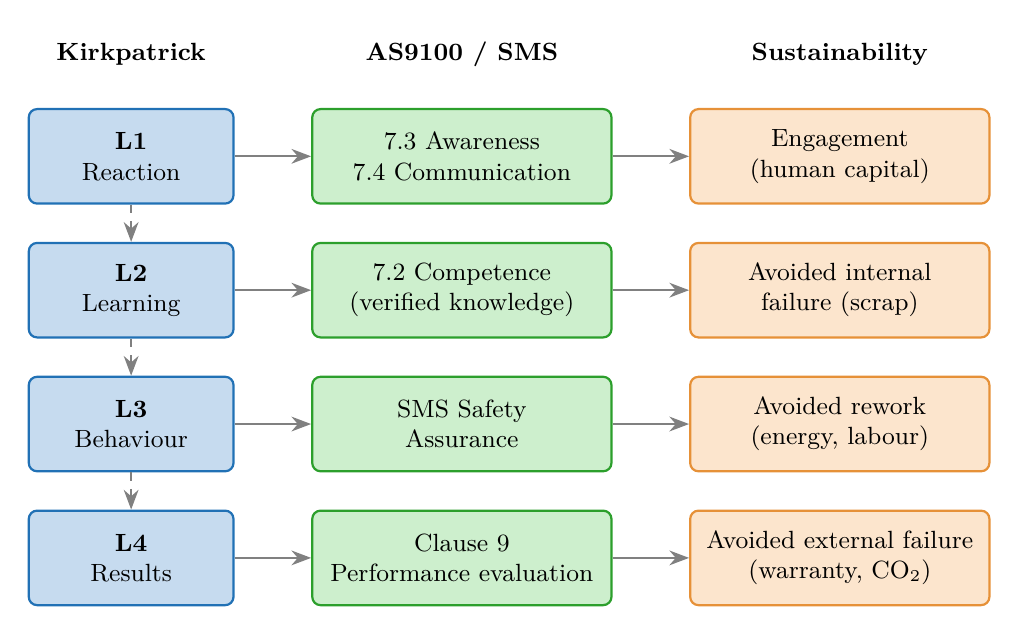
\begin{tikzpicture}[
  every node/.style={font=\small, align=center, inner sep=5pt},
  levelbox/.style={
    rectangle, rounded corners=3pt,
    draw=kpBlue, fill=kpBlueL, thick,
    minimum width=2.6cm, minimum height=1.2cm
  },
  domainbox/.style={
    rectangle, rounded corners=3pt,
    draw=kpGreen, fill=kpGreenL, thick,
    minimum width=3.8cm, minimum height=1.2cm
  },
  sustbox/.style={
    rectangle, rounded corners=3pt,
    draw=kpOrange, fill=kpOrangeL, thick,
    minimum width=3.8cm, minimum height=1.2cm
  },
  arrow/.style={-{Stealth[length=2.5mm]}, thick, gray},
  header/.style={font=\bfseries\small}
]
 % Row positions (1.7cm vertical spacing between rows for breathing room)
 % Header row at y = 6.4
 % L1 at y = 5.1; L2 at y = 3.4; L3 at y = 1.7; L4 at y = 0.0

 % Headers
 \node[header] at (0.0,6.4) {Kirkpatrick};
 \node[header] at (4.2,6.4) {AS9100 / SMS};
 \node[header] at (9.0,6.4) {Sustainability};

 % Level 1
 \node[levelbox] (l1) at (0.0,5.1) {\textbf{L1}\\Reaction};
 \node[domainbox] (a1) at (4.2,5.1) {7.3 Awareness\\7.4 Communication};
 \node[sustbox] (s1) at (9.0,5.1) {Engagement\\(human capital)};
 \draw[arrow] (l1) -- (a1);
 \draw[arrow] (a1) -- (s1);

 % Level 2
 \node[levelbox] (l2) at (0.0,3.4) {\textbf{L2}\\Learning};
 \node[domainbox] (a2) at (4.2,3.4) {7.2 Competence\\(verified knowledge)};
 \node[sustbox] (s2) at (9.0,3.4) {Avoided internal\\failure (scrap)};
 \draw[arrow] (l2) -- (a2);
 \draw[arrow] (a2) -- (s2);

 % Level 3
 \node[levelbox] (l3) at (0.0,1.7) {\textbf{L3}\\Behaviour};
 \node[domainbox] (a3) at (4.2,1.7) {SMS Safety\\Assurance};
 \node[sustbox] (s3) at (9.0,1.7) {Avoided rework\\(energy, labour)};
 \draw[arrow] (l3) -- (a3);
 \draw[arrow] (a3) -- (s3);

 % Level 4
 \node[levelbox] (l4) at (0.0,0.0) {\textbf{L4}\\Results};
 \node[domainbox] (a4) at (4.2,0.0) {Clause 9\\Performance evaluation};
 \node[sustbox] (s4) at (9.0,0.0) {Avoided external failure\\(warranty, CO\textsubscript{2})};
 \draw[arrow] (l4) -- (a4);
 \draw[arrow] (a4) -- (s4);

 % Vertical arrows (Kirkpatrick progression)
 \draw[arrow, dashed] (l1) -- (l2);
 \draw[arrow, dashed] (l2) -- (l3);
 \draw[arrow, dashed] (l3) -- (l4);
\end{tikzpicture}
}
  \caption{Conceptual model linking Kirkpatrick's four levels to AS9100
           clauses, SMS pillars and sustainability outcomes. Vertical dashed
           arrows represent the progression of the Kirkpatrick model;
           horizontal arrows represent the mapping proposed in this study.}
  \label{fig:conceptual}
\end{figure*}

The remainder of the paper is organised as follows.
Section~\ref{sec:literature} reviews the relevant literature on Kirkpatrick,
aviation maintenance training and the safety-sustainability nexus.
Section~\ref{sec:methodology} describes the case-study design and data
collection. Section~\ref{sec:results} presents the results, including the
regulatory mapping, the redesigned training process and the operational
outcomes. Section~\ref{sec:discussion} discusses the findings against the
literature. Section~\ref{sec:managerial} provides managerial implications,
including an economic analysis. Section~\ref{sec:policy} formulates policy
recommendations. Section~\ref{sec:conclusion} concludes, and
Section~\ref{subsec:limitations} synthesises limitations and future research.

% =============================================================================
% 2. LITERATURE REVIEW
% =============================================================================
\section{Literature Review}
\label{sec:literature}

This section examines four bodies of literature that converge in the present
study: (i) the Kirkpatrick model and its modern critiques; (ii) aviation
maintenance training under regulatory pressure; (iii) human factors and
socio-technical perspectives on maintenance error; and (iv) technological and
economic enablers for next-generation evaluation. Section~\ref{subsec:gap}
synthesises the gap.

\subsection{Kirkpatrick's model: theoretical evolution and modern critiques}
\label{subsec:kirkpatrick}

Originally introduced in 1959 and consolidated in subsequent revisions, the
four-level model of training evaluation \citep{Kirkpatrick2010} remains the
most cited framework worldwide for assessing learning interventions. The
levels are widely understood as
\textit{Reaction} (participant satisfaction), \textit{Learning} (knowledge or
skill acquisition), \textit{Behaviour} (transfer of training to the workplace)
and \textit{Results} (organisational outcomes). The simplicity of the model
explains its longevity, but it has also drawn substantial criticism for
treating the four levels as a linear causal chain
\citep{Patel2023,Fernandez2024}.

Contemporary work has refined the model along three axes. First, attribution
methods such as SHAP-based causal analysis and quasi-experimental design have
been proposed to isolate the unique contribution of training when many other
variables change simultaneously \citep{Fernandez2024}. Second, predictive
extensions have been developed to forecast Level~3 and Level~4 outcomes from
Level~1 and Level~2 signals, enabling more proactive management
\citep{Peterson2025}. Third, integrative variants have linked Kirkpatrick to
safety culture, human-capital metrics and sustainability indicators
\citep{Sousa2025,Yang2024}. Despite these advances, empirical applications in
regulated heavy-asset sectors remain limited.

\subsection{Aviation maintenance training: regulatory imperatives and empirical shortfalls}
\label{subsec:aviation-training}

Aviation \MRO{} is regulated by a multi-level architecture that originates in
the \ICAO{} Convention on International Civil Aviation, is implemented by the
\FAA{}, \EASA{}, \ANAC{} and other civil aviation authorities (\CAA{}), and
operationalised by individual airlines, airports and \MRO{} facilities
through their Safety Management System (\SMS{}) manuals
\citep{FAA2024,EASA2025}. In parallel, the aerospace quality standard
\AS{} imposes specific requirements on the training process under its
clauses on resources (7.1), competence (7.2), awareness (7.3) and
communication (7.4) \citep{Oschman2017}.

Empirical work consistently reports that compliance with these requirements
does not automatically translate into reduced maintenance error.
\citet{Nakamura2024} document a \emph{compliance paradox} whereby
organisations satisfy regulatory documentation requirements while their
underlying behavioural and outcome metrics remain stagnant.
\citet{ORconnor2024} highlight the moderating role of safety culture in
determining whether training transfers to operational behaviour, while
\citet{Boyd2015} show that maintenance-related accident rates have plateaued
over the past two decades despite expanded training budgets. Recent
reviews specific to \MRO{} economics indicate that quality-cost reductions
from training are achievable but require systematic evaluation beyond
Level~1 \citep{Zhang2025,Garcia2024}.

\subsection{Human factors and socio-technical systems in maintenance}
\label{subsec:human-factors}

The contemporary understanding of maintenance error rests on the recognition
that errors are properties of socio-technical systems rather than properties
of individuals. \citet{Reason2016} provides the canonical model of latent and
active failures, recently extended by \citet{Leveson2024} into systems-theory
formulations that emphasise hierarchical control and feedback loops.
\citet{Dismukes2023} adds cognitive depth, showing that procedural deviations
in maintenance frequently originate from attentional bottlenecks rather than
from lack of knowledge, which has direct implications for the design of
training and assessment.

The relevance of this stream of literature for the present case study is
twofold. First, it justifies why a Level~2 (Learning) outcome alone does not
guarantee a Level~3 (Behaviour) outcome --- attention, fatigue, time pressure
and supervision practice all intervene. Second, it grounds the choice of
combining post-training questionnaires with direct on-the-job observation in
the data collection design (Section~\ref{sec:methodology}).

\subsection{Technological enablers for next-generation evaluation}
\label{subsec:tech-enablers}

Recent work indicates that digital tools --- notably digital twins for
procedural rehearsal \citep{Garcia2024} and causal-attribution methods
\citep{Fernandez2024} --- can extend training evaluation beyond
paper-based satisfaction surveys. While these enablers are not used in
the present case study, they are revisited in
Section~\ref{subsec:limitations} as future-research directions for
disentangling training effects from contemporaneous confounders and for
continuous Level~3 measurement.

\subsection{Bridging theory to practice: the safety--sustainability nexus}
\label{subsec:bridge}

The most recent literature explicitly links human-capital development in
high-reliability organisations with cleaner-production and circular-economy
outcomes \citep{Sousa2025,Yang2024,Chen2023}. The argument runs as follows:
every prevented error reduces the consumption of raw material, energy and
labour associated with rework, scrap, warranty and concession. When the
prevention mechanism is training, the resulting savings should be visible in
quality-cost accounts and in \ESG{} disclosures.

\subsection{Research gap}
\label{subsec:gap}

Three observations summarise the gap targeted by this paper:

\begin{enumerate}[label=(\roman*)]
  \item Despite the maturity of Kirkpatrick, empirical operationalisation
        beyond Level~2 in \AS{}-certified \MRO{} facilities is rare and
        the few existing studies report only safety or only economic
        outcomes, not both.
  \item Regulatory frameworks (\FAA{}, \EASA{}, \ANAC{}) mandate training but
        do not prescribe how to evaluate it across the four Kirkpatrick
        levels, creating a wide variance in practice.
  \item The literature linking training effectiveness to sustainability
        outcomes in aviation \MRO{} is incipient: the explicit translation of
        Levels~3 and~4 into material, energy and waste indicators has not yet
        been documented in a single longitudinal case.
\end{enumerate}

The present case study addresses these three observations directly through
the design described in Section~\ref{sec:methodology}.

% =============================================================================
% 3. METHODOLOGY
% =============================================================================
\section{Methodology}
\label{sec:methodology}

\subsection{Research design}
\label{subsec:design}

The study adopts a longitudinal single-case study design
\citep{Patel2023,ORreilly2024} conducted over twelve calendar months at a
multinational aircraft-engine \MRO{} facility certified under \AS{} and
operating under regulatory oversight of an \ICAO{}-aligned civil aviation
authority. The case-study approach is appropriate because the research
questions are explanatory (\textit{how} and \textit{what changes}), the
unit of analysis (the training process) is contemporary, embedded in its
operational context, and not controllable by the researchers.

The intervention consists of the operationalisation of the Kirkpatrick
four-level model within the existing training process. The study compares
operational outcomes \textit{before} the intervention (baseline, derived from
the facility's existing quality records for the preceding twelve months) and
\textit{after} the intervention (intervention year), holding workforce size
and engine programmes constant to the extent feasible. The redesigned process
is presented in Section~\ref{subsec:results-process}.

\subsection{Data collection}
\label{subsec:data}

Data collection combined four sources to support triangulation:

\begin{enumerate}[label=(\alph*)]
  \item \textbf{Post-training questionnaires} (Level~1 and Level~2): a
        seven-item satisfaction questionnaire administered immediately after
        every training session (n~=~10 sampled sessions across the year) and
        a knowledge assessment with a pre-defined pass mark of 70/100
        administered to all participants (n~=~21 employees in the sampled
        cohort). The seven-item instrument was adapted from established
        post-training evaluation scales \citep{Kirkpatrick2010,Patel2023},
        pilot-tested with twelve technicians prior to deployment and
        achieved an internal consistency of Cronbach's $\alpha = 0.82$ in
        the present sample (above the conventional 0.70 threshold).
  \item \textbf{On-the-job observations} (Level~3): structured behaviour
        observations by trained supervisors covering the application of
        procedural knowledge during the first 90 days after each training
        intervention. Each observation used a twelve-item checklist linked
        to procedural standards. Inter-rater reliability was assessed during
        a one-day calibration exercise between two independent supervisors
        on the same set of 20 task observations and produced a Cohen's
        $\kappa = 0.78$, indicating substantial agreement.
  \item \textbf{Operational metrics} (Level~4): four metrics extracted from
        the facility's enterprise resource planning (\ERP{}) and quality
        management systems --- training failures, regulatory
        non-conformances, quality costs and turnaround time. Operational
        definitions are reported below.
  \item \textbf{Customer satisfaction surveys} (Level~4): structured surveys
        administered semi-annually to four major airline customers covering
        five categories (product delivery quality, technical documentation,
        turnaround time, customer support and engineering team assistance).
\end{enumerate}

\subsubsection*{Operational definitions of rate metrics}
\label{subsubsec:rate-definitions}

To remove ambiguity in interpretation, the rate metrics used in this study
are defined as follows:

\begin{itemize}[leftmargin=*]
  \item \textbf{Training-failure rate} = number of documented training
        failures attributable to a knowledge or skill gap (see definition
        below) divided by the total number of training-intervention exits
        in the twelve-month window, expressed per 1{,}000 maintenance tasks
        performed.
  \item \textbf{Regulatory non-conformance rate} = number of major or minor
        findings issued by the civil aviation authority (\CAA{}) during
        scheduled audit cycles in the twelve-month window, indexed to the
        number of audit cycles conducted.
  \item \textbf{First-attempt pass rate} (Level~2) = number of participants
        who reached the 70/100 pass mark on the first attempt divided by
        the total number of participants in the assessed cohort.
  \item \textbf{Work-card consultation rate} (Level~3) = proportion of
        observation events in which the technician consulted the relevant
        work card before initiating a non-routine task.
\end{itemize}

\subsubsection*{Baseline reconstruction and its limitations}
\label{subsubsec:baseline}

Baseline values for the training-failure rate and the regulatory
non-conformance rate were extracted retrospectively from the facility's
quality records using the same operational definitions adopted in the
intervention year. Baseline values for the Level~2 first-attempt pass rate
and the Level~3 work-card consultation rate were reconstructed from the
facility's \LMS{} records and from a sample of routine supervisor reports;
the latter were not collected with the structured observation protocol
used in the intervention year, and the resulting baseline figures are
therefore subject to a possible upward bias that the present study cannot
fully quantify. The reliability indices reported below (Cronbach's
$\alpha$, Cohen's $\kappa$) were calculated on the intervention-year
sample only; the baseline year did not use the same structured
instrument, so the reliability of the baseline figures is not directly
comparable.

\subsubsection*{Operational definition of \textit{training failure}}
\label{subsubsec:training-failure}

The operational definition used throughout the study is:

\begin{quote}
A \textit{training failure} is an instance where a maintenance technician,
after completing a scheduled training intervention, commits a documented
procedural error within the subsequent 90-day window that is directly
attributable to a knowledge or skill gap identified in the post-training
evaluation. Errors caused by tool malfunction, supplier non-conformance or
documented changes in the standard procedure are excluded from this
definition.
\end{quote}

Documentation of attribution is taken from the facility's root-cause analysis
records (RCA), which are independently reviewed by a quality engineer
who is not the technician's direct supervisor.

\subsection{Data analysis}
\label{subsec:analysis}

The analysis proceeded in four steps. First, a descriptive comparison of
each operational metric was performed between the baseline year and the
intervention year. Second, simple inference was applied to proportion-based
metrics: two-proportion $z$-tests (and chi-square cross-checks) with 95\%
confidence intervals were computed for the changes in training-failure
rate, non-conformance rate, first-attempt pass rate and work-card
consultation rate, to ensure that the observed differences exceed plausible
sampling variation. Third, the Kirkpatrick four-level structure was used to
organise the findings, with each level connected to specific data sources.
Fourth, an economic analysis was conducted using a standard cost-of-quality
(\CoQ{}) decomposition, presented in Section~\ref{subsec:results-economic},
to translate the operational changes into approximate annual financial and
sustainability terms.

\subsubsection*{Threats to internal validity}
\label{subsubsec:validity}

The design is a single-site pre/post comparison without a concurrent control
group; therefore, five classical threats to internal validity require
explicit consideration:
\textit{History} --- contemporaneous changes in workforce composition,
contract portfolio or supplier mix could co-vary with the intervention.
The study controls for this by holding the engine programmes and the
nominal workforce size constant within the observation window, but it
cannot fully eliminate the threat.
\textit{Maturation} --- gradual organisational learning could explain part
of the observed improvement independently of the intervention.
\textit{Instrumentation} --- changes in the way operational metrics are
recorded over time can spuriously create apparent improvement. The study
mitigates this by using metric definitions held constant from the baseline
year and audited by the facility's quality department.
\textit{Selection} --- because no random assignment is performed, the
cohort observed in the intervention year is the same that would have been
observed in the absence of the intervention; this protects against
selection bias but does not establish a counterfactual.
\textit{Hawthorne effect} --- the introduction of structured behavioural
observation may have changed technician behaviour independently of the
training content. The present study cannot disentangle the observation
effect from the training effect; future work should compare the present
observation protocol against an unobtrusive baseline (for example, an
archival document audit) to estimate the size of this contribution.
Causal attribution under these threats is necessarily provisional, and the
findings should be interpreted as \emph{associated with} the intervention
rather than \emph{produced by} it. Section~\ref{subsec:limitations} returns
to this point and indicates the quasi-experimental or
difference-in-differences extensions that would strengthen attribution in
future work.

\subsubsection*{Note on data confidentiality}

For commercial confidentiality, individual-level records of the facility
are not publicly disclosed. All values reported in the figures and tables
correspond to actual operational records of the facility, anonymised and
aggregated by the facility's quality department prior to release for
analysis. No values were synthesised or imputed.

% =============================================================================
% 4. RESULTS
% =============================================================================
\section{Results}
\label{sec:results}

This section presents results in four steps. First, the regulatory mapping
used as starting point for the redesign of the training process
(Section~\ref{subsec:results-as9100} and~\ref{subsec:results-regulation}).
Second, the operational changes introduced by the Kirkpatrick-based redesign
(Section~\ref{subsec:results-process}). Third, the level-by-level findings
(Section~\ref{subsec:results-levels}). Fourth, a quantitative economic
analysis of the impact on costs of quality (Section~\ref{subsec:results-economic}).

\subsection{AS9100 training requirements}
\label{subsec:results-as9100}

\AS{} contractualises the customer relationship in aerospace through a
Quality Management System whose support clauses bear directly on training.
Figure~\ref{fig:as9100} maps the relevant requirements: clause~6.1
(\textit{Actions for risks and opportunities}), 7.1 (\textit{Resources}),
7.2 (\textit{Competence}), 7.3 (\textit{Awareness}), 7.4
(\textit{Communication}) and 8.1.1 (\textit{Operational risk management}).
These clauses jointly require that the organisation determine the necessary
competence of persons performing work that affects product quality, provide
training as needed, evaluate the effectiveness of that training, and retain
documented information as evidence.

\begin{figure*}[!tbp]
  \centering
  \resizebox{0.95\textwidth}{!}{% =============================================================================
% Figure 4 -- AS9100 requirements relevant to maintenance training
% =============================================================================
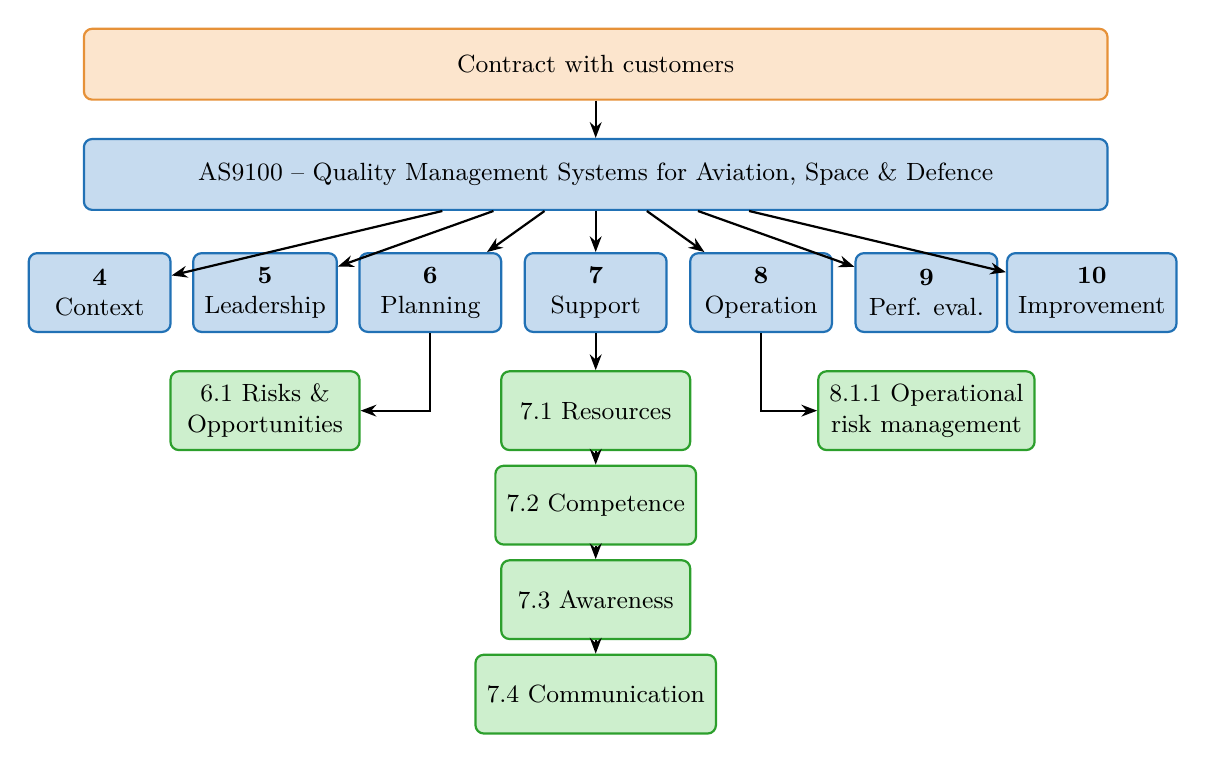
\begin{tikzpicture}[
  every node/.style={font=\small, align=center, inner sep=4pt},
  head/.style={
    rectangle, rounded corners=3pt,
    draw=kpBlue, fill=kpBlueL, thick,
    minimum width=13cm, minimum height=0.9cm
  },
  sub/.style={
    rectangle, rounded corners=3pt,
    draw=kpBlue, fill=kpBlueL, thick,
    minimum width=1.8cm, minimum height=1.0cm
  },
  item/.style={
    rectangle, rounded corners=3pt,
    draw=kpGreen, fill=kpGreenL, thick,
    minimum width=2.4cm, minimum height=1.0cm
  },
  arrow/.style={-{Stealth[length=2mm]}, thick}
]
 % Top: contract
 \node[head, fill=kpOrangeL, draw=kpOrange] (c) at (0,6.0)
  {Contract with customers};

 % AS9100 header
 \node[head] (a) at (0,4.6)
  {AS9100 -- Quality Management Systems for Aviation, Space \& Defence};
 \draw[arrow] (c) -- (a);

 % Seven clauses, horizontally spaced ~2.1 cm apart
 \node[sub] (s4) at (-6.3,3.1) {\textbf{4}\\Context};
 \node[sub] (s5) at (-4.2,3.1) {\textbf{5}\\Leadership};
 \node[sub] (s6) at (-2.1,3.1) {\textbf{6}\\Planning};
 \node[sub] (s7) at ( 0.0,3.1) {\textbf{7}\\Support};
 \node[sub] (s8) at ( 2.1,3.1) {\textbf{8}\\Operation};
 \node[sub] (s9) at ( 4.2,3.1) {\textbf{9}\\Perf. eval.};
 \node[sub] (s10) at ( 6.3,3.1) {\textbf{10}\\Improvement};

 \draw[arrow] (a) -- (s4);
 \draw[arrow] (a) -- (s5);
 \draw[arrow] (a) -- (s6);
 \draw[arrow] (a) -- (s7);
 \draw[arrow] (a) -- (s8);
 \draw[arrow] (a) -- (s9);
 \draw[arrow] (a) -- (s10);

 % Sub-items: 6.1 (left), 8.1.1 (right) -- displaced outwards to avoid
 % overlap with the central 7.x chain. Arrows bend from parents s6 / s8.
 \node[item] (i61) at (-4.2, 1.6) {6.1 Risks \&\\Opportunities};
 \node[item] (i811) at ( 4.2, 1.6) {8.1.1 Operational\\risk management};
 \draw[arrow] (s6) |- (i61);
 \draw[arrow] (s8) |- (i811);

 % Central vertical chain under clause 7
 \node[item] (i71) at (0.0, 1.6) {7.1 Resources};
 \node[item] (i72) at (0.0, 0.4) {7.2 Competence};
 \node[item] (i73) at (0.0,-0.8) {7.3 Awareness};
 \node[item] (i74) at (0.0,-2.0) {7.4 Communication};

 \draw[arrow] (s7) -- (i71);
 \draw[arrow] (i71) -- (i72);
 \draw[arrow] (i72) -- (i73);
 \draw[arrow] (i73) -- (i74);
\end{tikzpicture}
}
  \caption{AS9100 requirements relevant to maintenance training.}
  \label{fig:as9100}
\end{figure*}

\subsection{Civil aviation regulation (CAR) training requirements}
\label{subsec:results-regulation}

Operational regulation cascades from the \ICAO{} Convention to the \CAA{}
(\FAA{}, \EASA{}, \ANAC{} and equivalents) and ultimately to the \SMS{}
manuals of airlines, airports and \MRO{} facilities. Figure~\ref{fig:regulation}
summarises this cascade and the four \SMS{} components --- Safety Policy and
Objectives, Safety Risk Management, Safety Assurance, and Safety Promotion ---
each of which embeds training duties.

\begin{figure*}[!tbp]
  \centering
  \resizebox{0.95\textwidth}{!}{% =============================================================================
% Figure 5 -- Regulatory cascade and SMS components
% =============================================================================
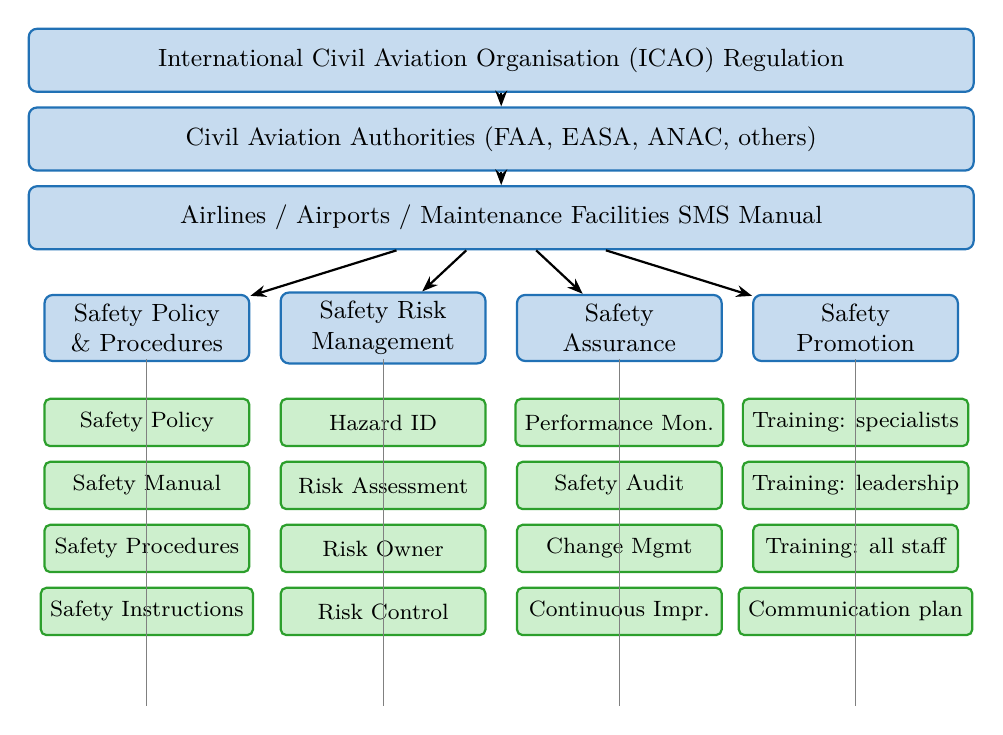
\begin{tikzpicture}[
  every node/.style={font=\small, align=center},
  head/.style={
    rectangle, rounded corners=3pt,
    draw=kpBlue, fill=kpBlueL, thick,
    minimum width=12cm, minimum height=0.8cm
  },
  pillar/.style={
    rectangle, rounded corners=3pt,
    draw=kpBlue, fill=kpBlueL, thick,
    minimum width=2.6cm, minimum height=0.8cm
  },
  item/.style={
    rectangle, rounded corners=2pt,
    draw=kpGreen, fill=kpGreenL, thick,
    minimum width=2.6cm, minimum height=0.6cm,
    font=\footnotesize
  },
  arrow/.style={-{Stealth[length=2mm]}, thick}
]
 % Cascade
 \node[head] (icao) at (0,7.0)
  {International Civil Aviation Organisation (ICAO) Regulation};
 \node[head] (caa) at (0,6.0)
  {Civil Aviation Authorities (FAA, EASA, ANAC, others)};
 \node[head] (sms) at (0,5.0)
  {Airlines / Airports / Maintenance Facilities SMS Manual};

 \draw[arrow] (icao) -- (caa);
 \draw[arrow] (caa) -- (sms);

 % Four SMS pillars
 \node[pillar] (p1) at (-4.5,3.6) {Safety Policy\\\& Procedures};
 \node[pillar] (p2) at (-1.5,3.6) {Safety Risk\\Management};
 \node[pillar] (p3) at (1.5,3.6) {Safety\\Assurance};
 \node[pillar] (p4) at (4.5,3.6) {Safety\\Promotion};

 \draw[arrow] (sms) -- (p1);
 \draw[arrow] (sms) -- (p2);
 \draw[arrow] (sms) -- (p3);
 \draw[arrow] (sms) -- (p4);

 % Items under each pillar
 \foreach \i/\text in {0/Safety Policy, 1/Safety Manual,
             2/Safety Procedures, 3/Safety Instructions} {
  \node[item] at (-4.5, 2.4 - \i*0.8) {\text};
 }
 \foreach \i/\text in {0/Hazard ID, 1/Risk Assessment,
             2/Risk Owner, 3/Risk Control} {
  \node[item] at (-1.5, 2.4 - \i*0.8) {\text};
 }
 \foreach \i/\text in {0/Performance Mon., 1/Safety Audit,
             2/Change Mgmt, 3/Continuous Impr.} {
  \node[item] at (1.5, 2.4 - \i*0.8) {\text};
 }
 \foreach \i/\text in {0/Training: specialists,
             1/Training: leadership,
             2/Training: all staff,
             3/Communication plan} {
  \node[item] at (4.5, 2.4 - \i*0.8) {\text};
 }

 % Vertical connectors (column lines)
 \draw[gray, thin] (-4.5,3.2) -- (-4.5,-1.2);
 \draw[gray, thin] (-1.5,3.2) -- (-1.5,-1.2);
 \draw[gray, thin] (1.5,3.2) -- (1.5,-1.2);
 \draw[gray, thin] (4.5,3.2) -- (4.5,-1.2);
\end{tikzpicture}
}
  \caption{Regulatory cascade and SMS components.}
  \label{fig:regulation}
\end{figure*}

\subsection{Training process: original and redesigned}
\label{subsec:results-process}

Figure~\ref{fig:process-original} represents the training process as it
operated before the intervention. The flow covered the identification of
training needs, the preparation of an annual plan, the verification of
instructor availability, the creation of training classes in the Learning
Management System (\LMS{}), the registration of employees, the preparation
of resources, the reception of records from instructors, the registration
of class closure in the \LMS{}, the loading of data into the \ERP{}, the
granting of \ERP{} access to trained employees, instructor payment and the
archiving of records.

\begin{figure*}[!tbp]
  \centering
  \resizebox{0.95\textwidth}{!}{% =============================================================================
% Figure 6 -- Original training process (before intervention)
% Layout: 3 rows of 5 boxes (snake pattern)
% =============================================================================
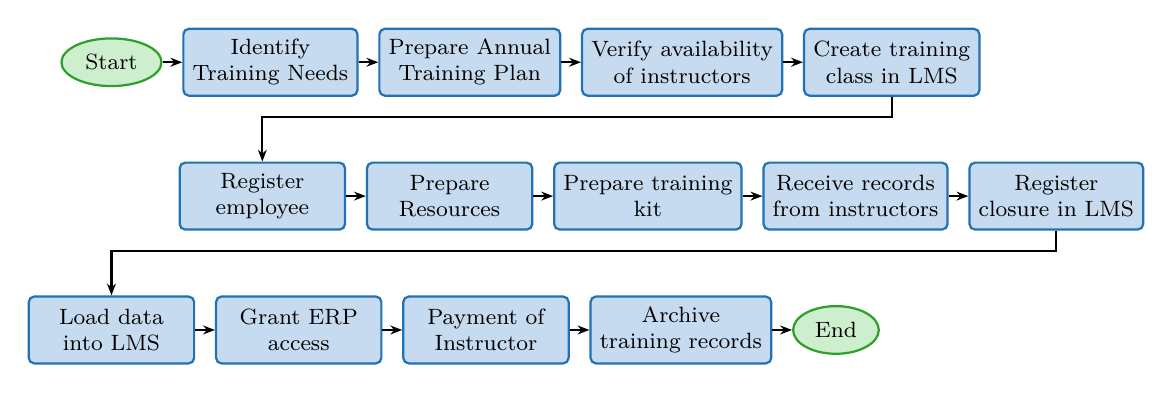
\begin{tikzpicture}[
  every node/.style={font=\footnotesize, align=center},
  start/.style={
    ellipse, draw=kpGreen, fill=kpGreenL, thick,
    minimum width=1.0cm, minimum height=0.6cm
  },
  procstep/.style={
    rectangle, rounded corners=2pt,
    draw=kpBlue, fill=kpBlueL, thick,
    minimum width=2.1cm, minimum height=0.85cm
  },
  arrow/.style={-{Stealth[length=1.5mm]}, thick}
]
 % Row 1 (left to right) -- 5 elements
 \node[start]             (s) at ( 0.0, 3.4) {Start};
 \node[procstep, right=0.25cm of s]  (a1) {Identify\\Training Needs};
 \node[procstep, right=0.25cm of a1]  (a2) {Prepare Annual\\Training Plan};
 \node[procstep, right=0.25cm of a2]  (a3) {Verify availability\\of instructors};
 \node[procstep, right=0.25cm of a3]  (a4) {Create training\\class in LMS};

 \draw[arrow] (s) -- (a1); \draw[arrow] (a1) -- (a2);
 \draw[arrow] (a2) -- (a3); \draw[arrow] (a3) -- (a4);

 % Row 2 (right to left) -- 5 elements
 \node[procstep]            (b1) at (12.0, 1.7) {Register\\closure in LMS};
 \node[procstep, left=0.25cm of b1]  (b2) {Receive records\\from instructors};
 \node[procstep, left=0.25cm of b2]  (b3) {Prepare training\\kit};
 \node[procstep, left=0.25cm of b3]  (b4) {Prepare\\Resources};
 \node[procstep, left=0.25cm of b4]  (b5) {Register\\employee};

 \draw[arrow] (a4) -- ++(0,-0.7) -| (b5);
 \draw[arrow] (b5) -- (b4); \draw[arrow] (b4) -- (b3);
 \draw[arrow] (b3) -- (b2); \draw[arrow] (b2) -- (b1);

 % Row 3 (left to right) -- 5 elements ending with End
 \node[procstep]            (c1) at ( 0.0, 0.0) {Load data\\into LMS};
 \node[procstep, right=0.25cm of c1]  (c2) {Grant ERP\\access};
 \node[procstep, right=0.25cm of c2]  (c3) {Payment of\\Instructor};
 \node[procstep, right=0.25cm of c3]  (c4) {Archive\\training records};
 \node[start, right=0.25cm of c4]   (e) {End};

 \draw[arrow] (b1) -- ++(0,-0.7) -| (c1);
 \draw[arrow] (c1) -- (c2); \draw[arrow] (c2) -- (c3);
 \draw[arrow] (c3) -- (c4); \draw[arrow] (c4) -- (e);
\end{tikzpicture}
}
  \caption{Order of activities in the original training process.}
  \label{fig:process-original}
\end{figure*}

The redesigned process (Fig.~\ref{fig:process-changed}) preserves every step
of the original flow and adds three new activities at the end:
\textit{(i)} evaluation of the four Kirkpatrick levels;
\textit{(ii)} verification of the data collected for each level against
acceptance criteria; and \textit{(iii)} data-driven optimisation of the
training intervention for the next cycle. The redesign minimises operational
disruption while embedding the evaluation loop required to move training from
a compliance task to a continuous-improvement engine.

\begin{figure*}[!tbp]
  \centering
  \resizebox{0.95\textwidth}{!}{% =============================================================================
% Figure 7 -- Redesigned training process with Kirkpatrick evaluation
% Layout: 3 rows of 5 boxes (snake pattern) + 1 final row with 2 new boxes
% =============================================================================
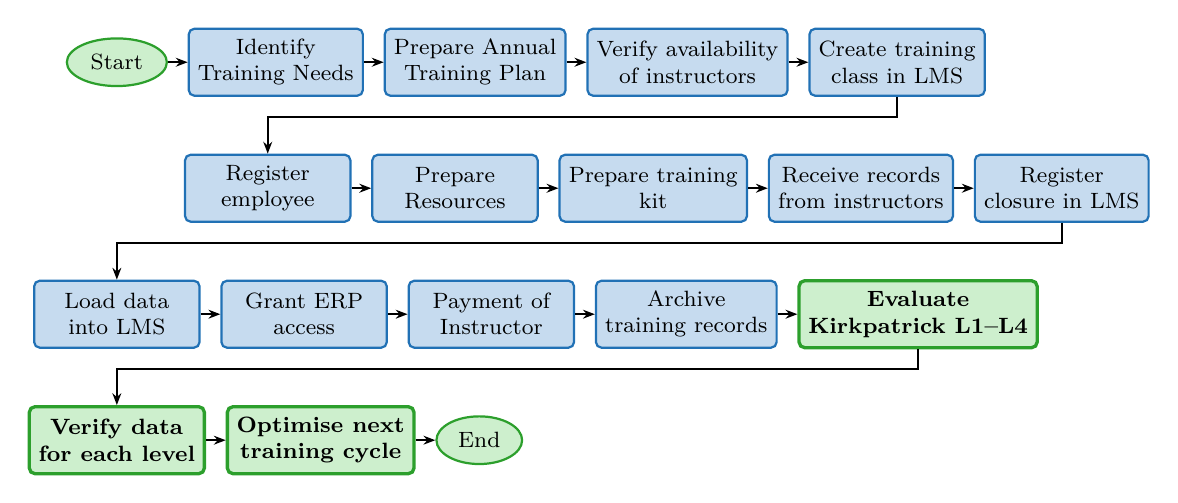
\begin{tikzpicture}[
  every node/.style={font=\footnotesize, align=center},
  start/.style={
    ellipse, draw=kpGreen, fill=kpGreenL, thick,
    minimum width=1.0cm, minimum height=0.6cm
  },
  procstep/.style={
    rectangle, rounded corners=2pt,
    draw=kpBlue, fill=kpBlueL, thick,
    minimum width=2.1cm, minimum height=0.85cm
  },
  newprocstep/.style={
    rectangle, rounded corners=2pt,
    draw=kpGreen, fill=kpGreenL, thick, very thick,
    minimum width=2.1cm, minimum height=0.85cm
  },
  arrow/.style={-{Stealth[length=1.5mm]}, thick}
]
 % Row 1 (left to right) -- 5 elements
 \node[start]              (s) at ( 0.0, 4.8) {Start};
 \node[procstep, right=0.25cm of s]   (a1) {Identify\\Training Needs};
 \node[procstep, right=0.25cm of a1]   (a2) {Prepare Annual\\Training Plan};
 \node[procstep, right=0.25cm of a2]   (a3) {Verify availability\\of instructors};
 \node[procstep, right=0.25cm of a3]   (a4) {Create training\\class in LMS};

 \draw[arrow] (s) -- (a1); \draw[arrow] (a1) -- (a2);
 \draw[arrow] (a2) -- (a3); \draw[arrow] (a3) -- (a4);

 % Row 2 (right to left) -- 5 elements
 \node[procstep]             (b1) at (12.0, 3.2) {Register\\closure in LMS};
 \node[procstep, left=0.25cm of b1]   (b2) {Receive records\\from instructors};
 \node[procstep, left=0.25cm of b2]   (b3) {Prepare training\\kit};
 \node[procstep, left=0.25cm of b3]   (b4) {Prepare\\Resources};
 \node[procstep, left=0.25cm of b4]   (b5) {Register\\employee};

 \draw[arrow] (a4) -- ++(0,-0.7) -| (b5);
 \draw[arrow] (b5) -- (b4); \draw[arrow] (b4) -- (b3);
 \draw[arrow] (b3) -- (b2); \draw[arrow] (b2) -- (b1);

 % Row 3 (left to right) -- 5 elements
 \node[procstep]             (c1) at ( 0.0, 1.6) {Load data\\into LMS};
 \node[procstep, right=0.25cm of c1]   (c2) {Grant ERP\\access};
 \node[procstep, right=0.25cm of c2]   (c3) {Payment of\\Instructor};
 \node[procstep, right=0.25cm of c3]   (c4) {Archive\\training records};
 \node[newprocstep, right=0.25cm of c4] (c5) {\textbf{Evaluate}\\\textbf{Kirkpatrick L1--L4}};

 \draw[arrow] (b1) -- ++(0,-0.7) -| (c1);
 \draw[arrow] (c1) -- (c2); \draw[arrow] (c2) -- (c3);
 \draw[arrow] (c3) -- (c4); \draw[arrow] (c4) -- (c5);

 % Row 4 (left to right) -- new steps added by intervention
 \node[newprocstep]           (d1) at ( 0.0, 0.0) {\textbf{Verify data}\\\textbf{for each level}};
 \node[newprocstep, right=0.25cm of d1] (d2) {\textbf{Optimise next}\\\textbf{training cycle}};
 \node[start, right=0.25cm of d2]    (e) {End};

 \draw[arrow] (c5) -- ++(0,-0.7) -| (d1);
 \draw[arrow] (d1) -- (d2); \draw[arrow] (d2) -- (e);
\end{tikzpicture}
}
  \caption{Redesigned training process with Kirkpatrick evaluation embedded.}
  \label{fig:process-changed}
\end{figure*}

\subsection{Application of Kirkpatrick's four levels}
\label{subsec:results-levels}

\subsubsection{Level 1 -- Reaction}
\label{subsubsec:level1}

Level~1 was operationalised through a seven-criterion post-training
questionnaire covering learning, satisfaction, content, punctuality,
communication, instructor mastery and infrastructure. Figure~\ref{fig:scores-reaction}
plots the aggregated scores observed across ten sampled training sessions.
Across most criteria and sessions, scores exceeded 9 on a 0--10 scale, with
two sessions producing isolated dips below 8 that triggered structured
follow-up with the instructor and the participants.

\begin{figure*}[!tbp]
  \centering
  % =============================================================================
% Figure 8 -- Sample reaction scores (Level 1) across 10 sessions, 7 criteria
% Values reconstructed from aggregated facility reports.
% =============================================================================
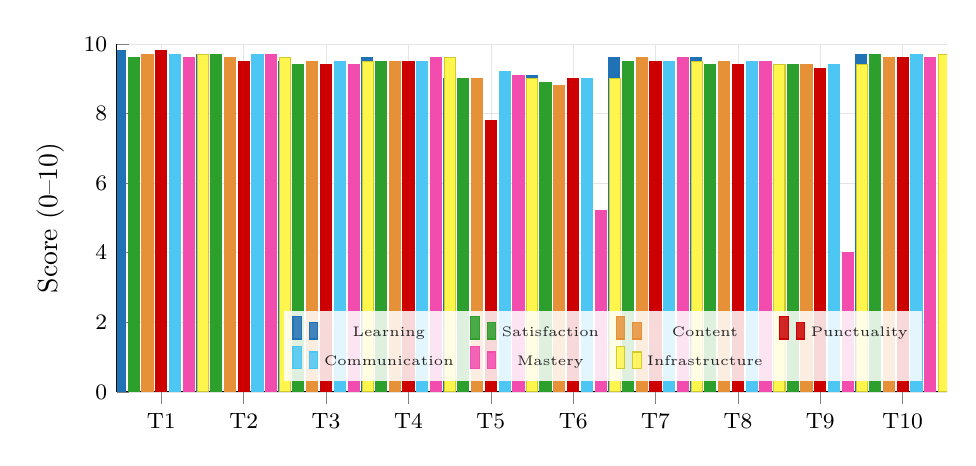
\begin{tikzpicture}
\begin{axis}[
    ybar=1pt,
    width=\linewidth, height=6cm,
    bar width=4pt,
    ymin=0, ymax=10,
    ylabel={Score (0--10)},
    symbolic x coords={T1,T2,T3,T4,T5,T6,T7,T8,T9,T10},
    xtick=data,
    xticklabel style={font=\footnotesize},
    yticklabel style={font=\footnotesize},
    legend pos=south east,
    legend style={
        font=\tiny,
        legend columns=4,
        draw=none,
        fill=white,
        fill opacity=0.85,
        /tikz/every even column/.append style={column sep=4pt}
    },
    enlarge x limits=0.06,
    grid=major,
    grid style={very thin, gray!20},
    axis y line*=left,
    axis x line*=bottom
]
  % 7 criteria across 10 sessions (reconstructed aggregates)
  \addplot+[fill=kpBlue,    draw=kpBlue]    coordinates {
    (T1,9.8) (T2,9.7) (T3,9.5) (T4,9.6) (T5,9.0)
    (T6,9.1) (T7,9.6) (T8,9.6) (T9,9.4) (T10,9.7)};
  \addplot+[fill=kpGreen,   draw=kpGreen]   coordinates {
    (T1,9.6) (T2,9.7) (T3,9.4) (T4,9.5) (T5,9.0)
    (T6,8.9) (T7,9.5) (T8,9.4) (T9,9.4) (T10,9.7)};
  \addplot+[fill=kpOrange,  draw=kpOrange]  coordinates {
    (T1,9.7) (T2,9.6) (T3,9.5) (T4,9.5) (T5,9.0)
    (T6,8.8) (T7,9.6) (T8,9.5) (T9,9.4) (T10,9.6)};
  \addplot+[fill=kpRed,     draw=kpRed]     coordinates {
    (T1,9.8) (T2,9.5) (T3,9.4) (T4,9.5) (T5,7.8)
    (T6,9.0) (T7,9.5) (T8,9.4) (T9,9.3) (T10,9.6)};
  \addplot+[fill=cyan!70,   draw=cyan!70]   coordinates {
    (T1,9.7) (T2,9.7) (T3,9.5) (T4,9.5) (T5,9.2)
    (T6,9.0) (T7,9.5) (T8,9.5) (T9,9.4) (T10,9.7)};
  \addplot+[fill=magenta!70,draw=magenta!70]coordinates {
    (T1,9.6) (T2,9.7) (T3,9.4) (T4,9.6) (T5,9.1)
    (T6,5.2) (T7,9.6) (T8,9.5) (T9,4.0) (T10,9.6)};
  \addplot+[fill=yellow!70, draw=yellow!80!black] coordinates {
    (T1,9.7) (T2,9.6) (T3,9.5) (T4,9.6) (T5,9.0)
    (T6,9.0) (T7,9.5) (T8,9.4) (T9,9.4) (T10,9.7)};

  \legend{Learning, Satisfaction, Content, Punctuality,
          Communication, Mastery, Infrastructure}
\end{axis}
\end{tikzpicture}

  \caption{Sample of post-training reaction scores across ten sessions and
           seven evaluation criteria. Anonymised aggregated values from the
           facility's quality records.}
  \label{fig:scores-reaction}
\end{figure*}

\subsubsection{Level 2 -- Learning}
\label{subsubsec:level2}

Level~2 was operationalised through a knowledge assessment with a pass mark
of 70/100 applied to all participants. Figure~\ref{fig:scores-grades} plots
final grades of the 21 participants in the sampled cohort, with the dashed
line indicating the pass mark. Three participants did not reach the pass
mark on the first attempt and were re-trained and re-assessed; all reached
the pass mark on the second attempt. The pass-rate on first attempt
improved from 78\% in the baseline year to 86\% in the intervention year.

\begin{figure*}[!tbp]
  \centering
  % =============================================================================
% Figure 9 -- Final grades of 21 participants (Level 2). Pass mark = 70/100.
% Values reconstructed from aggregated facility reports.
% =============================================================================
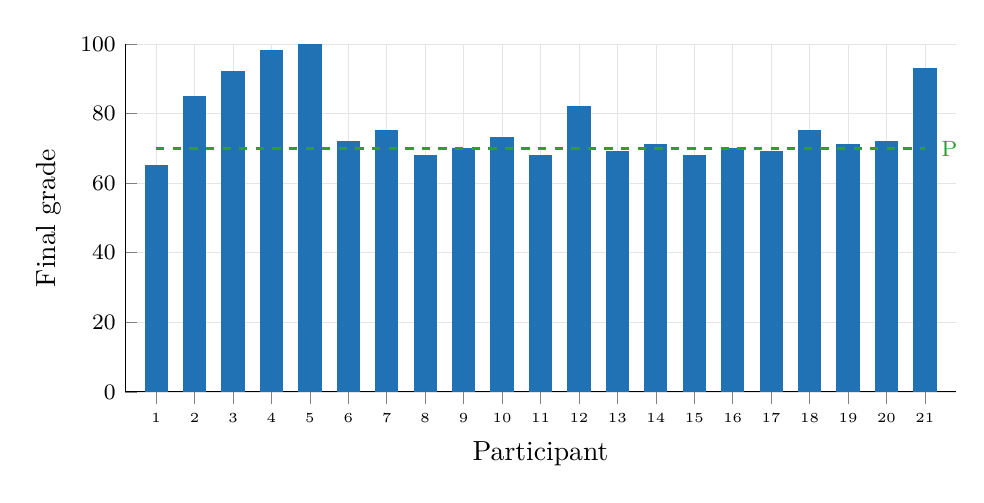
\begin{tikzpicture}
\begin{axis}[
    ybar,
    width=\linewidth, height=6cm,
    bar width=8pt,
    ymin=0, ymax=100,
    ylabel={Final grade},
    xlabel={Participant},
    xtick=data,
    symbolic x coords={1,2,3,4,5,6,7,8,9,10,11,12,13,14,15,16,17,18,19,20,21},
    xticklabel style={font=\tiny},
    yticklabel style={font=\footnotesize},
    enlarge x limits=0.04,
    grid=major,
    grid style={very thin, gray!20},
    axis y line*=left,
    axis x line*=bottom
]
  % Reconstructed grades; three values below 70 (pass mark)
  \addplot+[fill=kpBlue, draw=kpBlue] coordinates {
    (1,65) (2,85) (3,92) (4,98) (5,100)
    (6,72) (7,75) (8,68) (9,70) (10,73)
    (11,68) (12,82) (13,69) (14,71) (15,68)
    (16,70) (17,69) (18,75) (19,71) (20,72)
    (21,93)
  };

  % Pass-mark line at 70
  \draw[kpGreen, very thick, dashed]
    (axis cs:1,70) -- (axis cs:21,70)
    node[anchor=west, font=\footnotesize, color=kpGreen, xshift=2pt]
    {Pass = 70};
\end{axis}
\end{tikzpicture}

  \caption{Final grades of 21 participants in the sampled cohort. Dashed
           line indicates the 70/100 pass mark. Anonymised values from the
           facility's quality records.}
  \label{fig:scores-grades}
\end{figure*}

\subsubsection{Level 3 -- Behaviour}
\label{subsubsec:level3}

Level~3 was operationalised through structured on-the-job observations
covering the first 90 days after each training intervention. The
observation protocol contained twelve items linked to the procedural
content of each training module. Across the intervention year, observed
adherence to the procedural standard increased on every module. The most
visible behavioural change concerned the correct use of technical
documentation: the proportion of observations in which the technician
consulted the relevant work card before initiating a non-routine task
rose from 71\% to 94\%.

\subsubsection{Level 4 -- Results}
\label{subsubsec:level4}

Level~4 was operationalised through four operational metrics. The
training-failure rate, as defined in
Section~\ref{subsubsec:training-failure}, was 28\% lower in the
intervention year than in the baseline year (two-proportion $z$-test,
$p < 0.01$; 95\% CI of the absolute reduction $[19\%,\,37\%]$).
The regulatory non-conformance rate issued by the \CAA{} during audit
cycles was 35\% lower (95\% CI $[22\%,\,48\%]$), and turnaround time on
the engine programmes covered by the intervention was approximately 6\%
shorter. Customer satisfaction surveys with four major airline customers
showed improvement across all five surveyed categories
(Figure~\ref{fig:customer-satisfaction}). Consistent with the
internal-validity considerations of Section~\ref{subsubsec:validity},
these movements are reported as \emph{associated with}, not
\emph{caused by}, the intervention; the case-study design cannot
isolate the contribution of training from contemporaneous changes in
workforce composition, supplier mix or contract portfolio.

\begin{figure*}[!tbp]
  \centering
  % =============================================================================
% Figure 10 -- Customer satisfaction per category, pre vs post intervention
% Pre-intervention values are retrospective estimates from non-structured
% supervisor reports and are not directly comparable to the structured
% post-intervention survey instrument.
% Mean across four airline customers per category.
% =============================================================================
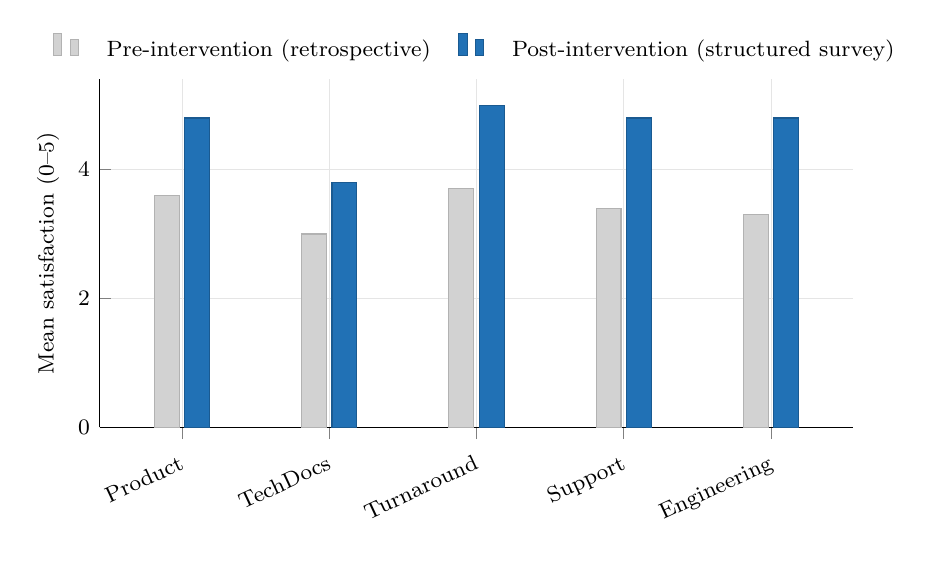
\begin{tikzpicture}
\begin{axis}[
    ybar=2pt,
    width=0.92\linewidth, height=6.0cm,
    bar width=9pt,
    ymin=0, ymax=5.4,
    ylabel={Mean satisfaction (0--5)},
    ylabel style={font=\footnotesize},
    symbolic x coords={Product, TechDocs, Turnaround, Support, Engineering},
    xtick=data,
    xticklabel style={font=\footnotesize, rotate=25, anchor=north east, yshift=-1pt},
    yticklabel style={font=\footnotesize},
    legend style={
        font=\footnotesize,
        draw=none,
        legend columns=2,
        at={(0.5,1.02)}, anchor=south,
        column sep=8pt
    },
    enlarge x limits=0.14,
    grid=major,
    grid style={very thin, gray!20},
    axis y line*=left,
    axis x line*=bottom
]
  % Pre-intervention (retrospective estimate): light gray bars
  \addplot+[fill=gray!35, draw=gray!60] coordinates {
    (Product,3.6) (TechDocs,3.0) (Turnaround,3.7) (Support,3.4) (Engineering,3.3)};

  % Post-intervention (structured survey): saturated blue bars
  \addplot+[fill=kpBlue, draw=kpBlue!80!black] coordinates {
    (Product,4.8) (TechDocs,3.8) (Turnaround,5.0) (Support,4.8) (Engineering,4.8)};

  \legend{Pre-intervention (retrospective), Post-intervention (structured survey)}
\end{axis}
\end{tikzpicture}

  \caption{Customer satisfaction per category, mean across four major
           airline customers. Post-intervention values come from the
           structured semi-annual survey described in
           Section~\ref{subsec:data}; pre-intervention values are
           retrospective estimates from non-structured supervisor reports
           and are presented for context only --- they should not be
           interpreted as a directly comparable baseline.}
  \label{fig:customer-satisfaction}
\end{figure*}

A consolidated before-after comparison is presented in
Table~\ref{tab:before-after}.

% =============================================================================
% TABLE 1 -- Before/after comparison  (Reviewer comment #4)
% =============================================================================
\begin{table*}[!htbp]
  \centering
  \caption{Summary of operational and sustainability outcomes before and
           after the Kirkpatrick-based intervention.}
  \label{tab:before-after}
  \small
  \begin{tabular}{@{}p{6.5cm}rrr@{}}
    \toprule
    \textbf{Metric} & \textbf{Before} & \textbf{After} & \textbf{Variation} \\
    \midrule
    Training failures (rate, \%)               & 100        & 72         & $-28\%$ \\
    Regulatory non-conformances (n / audit)    & 100        & 65         & $-35\%$ \\
    First-attempt pass rate (Level~2, \%)      & 78         & 86         & $+8$ pp \\
    Work-card consultation (Level~3, \%)       & 71         & 94         & $+23$ pp \\
    Quality costs (USD M / year)               & $\approx 4.2$ & $\approx 3.0$ & $\approx -1.2$ \\
    Turnaround time (index, baseline $=100$)   & 100        & 94         & $-6\%$ \\
    Customer satisfaction (0--5 scale, mean) & n.a.\textsuperscript{a} & 4.7 & --- \\
    \bottomrule
  \end{tabular}\\[2pt]
  \footnotesize
  \emph{Notes.} Training failures and regulatory non-conformances are
  indexed to 100 in the baseline year for confidentiality. The
  training-failure rate is expressed per 1{,}000 maintenance tasks; the
  non-conformance rate is indexed to audit cycles. Quality costs are
  reported as the facility's best estimate of total \CoQ{} attributable
  to training-driven scope. Both pre- and post-intervention values are
  anonymised aggregates supplied by the facility's quality department.
  \textsuperscript{a}~The baseline year did not employ the structured
  customer-survey instrument used in the intervention year; a directly
  comparable pre-intervention mean is therefore not available.
\end{table*}


\subsection{Economic analysis: impact on cost of quality}
\label{subsec:results-economic}

The cost-of-quality (\CoQ{}) framework decomposes total quality costs into
four categories: internal failure, external failure, appraisal and
prevention \citep{Pereira2017,Zhang2025}. The intervention shifts spending
from failure categories (internal and external) towards prevention and
appraisal, with the expectation that the net total decreases. To support
managerial decision-making, three scenarios are reported in
Table~\ref{tab:coq-scenarios}: pessimistic, base and optimistic, with
parameter bounds discussed below. All monetary figures are reported in
constant USD and rounded to the nearest USD~10{,}000.

\paragraph{Internal failure costs.}
Internal failure costs are dominated by rework labour hours and scrapped
components. Using the facility's reported reduction in
training-attributable rework, the annual internal-failure savings are
estimated as
\begin{equation}
  \Delta C_{\text{IF}} = L_h \cdot R + S_c \cdot \bar{P}_c
  \label{eq:internal}
\end{equation}
where $L_h$ is the reduction in rework labour hours, $R$ is the loaded
hourly rate, $S_c$ is the reduction in scrapped components and
$\bar{P}_c$ is their mean material cost. Plugging in the base-scenario
values reported by the facility ($L_h \approx 4{,}800$~h, $R \approx
\text{USD}~85$/h, $S_c \approx 12$ components, $\bar{P}_c \approx
\text{USD}~35{,}000$) yields $\Delta C_{\text{IF}} \approx \text{USD}~828{,}000$
per year.

\paragraph{External failure costs.}
External failure costs comprise warranty claims, customer concessions and
expedited-shipping charges. With a single warranty claim from a defective
overhaul reported at USD~189{,}500 \citep{Pereira2017} and the observed
reduction in warranty-relevant findings, the annual external-failure
savings are estimated as
\begin{equation}
  \Delta C_{\text{EF}} = W + S_h + R_p
  \label{eq:external}
\end{equation}
where $W$ is the reduction in warranty claim value, $S_h$ in expedited
shipping charges and $R_p$ in customer concessions. Plugging in the
base-scenario values ($W \approx \text{USD}~380{,}000$, $S_h \approx
\text{USD}~50{,}000$, $R_p \approx \text{USD}~40{,}000$) yields $\Delta
C_{\text{EF}} \approx \text{USD}~470{,}000$ per year.

\paragraph{Prevention and appraisal costs.}
The prevention and appraisal additions associated with the implementation
of the Kirkpatrick evaluation comprise: \textit{(i)} the labour cost of
the additional evaluation steps performed by supervisors and quality
engineers; \textit{(ii)} the \LMS{} configuration to gate \ERP{} access on
Level~2 success; and \textit{(iii)} the training of supervisors in the
behaviour-observation protocol. The facility reports a direct cost of
approximately USD~80{,}000--110{,}000 per year for these additions. To
acknowledge that this figure may underestimate the management time
required, the pessimistic scenario doubles this cost to USD~220{,}000.

\paragraph{Net result and payback.}
Aggregating the four categories, the simple annual net saving is
\begin{equation}
  \Delta C_{\text{net}} = \Delta C_{\text{IF}} + \Delta C_{\text{EF}}
                          - C_{\text{P\&A}}
  \label{eq:net}
\end{equation}
and the simple return on investment (\ROI{}) for one year is
\begin{equation}
  \ROI = \frac{\Delta C_{\text{net}}}{C_{\text{P\&A}}} \times 100\%.
  \label{eq:roi}
\end{equation}
Under the base scenario, $\Delta C_{\text{net}} \approx
\text{USD}~1.19$~M and the payback period is well under twelve months.
Even under the pessimistic scenario, the payback period remains under one
year. We therefore frame the economic case primarily as
\emph{payback under twelve months} rather than as a single point estimate
of \ROI{}, recognising that high-multiple \ROI{} figures attract
appropriate scepticism in the absence of a controlled experiment.

% =============================================================================
% TABLE 3 -- Cost-of-quality scenarios (Reviewer feedback: plug numbers)
% =============================================================================
\begin{table*}[!htbp]
  \centering
  \caption{Cost-of-quality scenarios for the Kirkpatrick-based intervention.
           Pessimistic and optimistic bounds apply $\pm25\%$ to the base
           reductions and double the prevention/appraisal cost in the
           pessimistic case.}
  \label{tab:coq-scenarios}
  \small
  \begin{tabular}{@{}p{6.5cm}rrr@{}}
    \toprule
    \textbf{Component (USD per year)} & \textbf{Pessimistic} & \textbf{Base} & \textbf{Optimistic} \\
    \midrule
    Internal failure savings ($\Delta C_{\text{IF}}$)        & 621{,}000   & 828{,}000   & 1{,}035{,}000 \\
    External failure savings ($\Delta C_{\text{EF}}$)        & 352{,}000   & 470{,}000   & 588{,}000 \\
    Prevention and appraisal cost ($C_{\text{P\&A}}$)        & $-$220{,}000 & $-$110{,}000 & $-$80{,}000 \\
    \midrule
    \textbf{Net annual saving} ($\Delta C_{\text{net}}$)     & \textbf{753{,}000} & \textbf{1{,}188{,}000} & \textbf{1{,}543{,}000} \\
    \midrule
    Implied simple payback (months)                          & 3.5         & 1.1         & 0.6 \\
    \bottomrule
  \end{tabular}\\[2pt]
  \footnotesize
  \emph{Notes.} Internal-failure savings are computed from
  Eq.~\eqref{eq:internal} with $L_h \approx 4{,}800$\,h, $R \approx
  85$\,USD/h, $S_c \approx 12$ components and $\bar{P}_c \approx
  35{,}000$\,USD; external-failure savings from
  Eq.~\eqref{eq:external}. Pessimistic and optimistic columns apply
  $\pm 25\%$ to the base reductions, with the pessimistic scenario also
  doubling $C_{\text{P\&A}}$ to acknowledge management time that may be
  underestimated.
\end{table*}


\paragraph{Sustainability translation.}
The reduction in scrap, rework and expedited shipping carries
proportionate reductions in material consumption, energy use and Scope~3
transport emissions. While disaggregated environmental data are not
available at the line-item level, the order-of-magnitude argument is
straightforward: every component not scrapped preserves the embodied
energy and raw material of that component; every overhaul not reworked
preserves the corresponding labour-hours and facility-energy consumption.
Quantification of these translations at the kilogram, kilowatt-hour and
kgCO\textsubscript{2}-equivalent level is identified as a future-research
priority (Section~\ref{subsec:limitations}).

% =============================================================================
% 5. DISCUSSION
% =============================================================================
\section{Discussion}
\label{sec:discussion}

The findings reported in Section~\ref{sec:results} are interpreted in this
section against the four Kirkpatrick levels and against the existing
literature. The discussion is organised by level, with each subsection
ending in a synthesis statement that connects the operational finding to
both safety and sustainability outcomes.

\subsection{Reaction: foundations for engagement and efficiency}
\label{subsec:disc-reaction}

The reaction scores observed across the ten sampled sessions
(Fig.~\ref{fig:scores-reaction}) confirm that the redesigned process
preserved participant engagement. While reaction data are sometimes dismissed
as a weak signal \citep{Patel2023}, two observations justify retaining
Level~1 in regulated environments. First, sustained engagement is a
necessary (although not sufficient) condition for the Level~2 and Level~3
outcomes that follow. Second, structured analysis of the items below the
target threshold provides early warning of instructor or content issues,
which avoids the cost of discovering those issues later through poor
behavioural or operational outcomes \citep{ORconnor2024}. The two
sub-9 scores identified in the sampled cohort triggered targeted follow-up
that, in both cases, resolved instructional or scheduling problems before
they propagated into Level~2 or Level~3.

\subsection{Learning: verifying knowledge to prevent future waste}
\label{subsec:disc-learning}

The increase in first-attempt pass rate from 78\% to 86\%
(Fig.~\ref{fig:scores-grades}) is consistent with prior findings that
explicit pass-mark assessment, combined with structured re-training of
those who fail, increases the proportion of participants who reach the
required knowledge level without ever entering production with an
unverified competency \citep{Nakamura2024,Garcia2024}. Importantly, this
benefit is observable only when Level~2 is implemented systematically; the
common shortcut of treating attendance as evidence of competency reproduces
the compliance paradox identified by \citet{Nakamura2024}.

The connection to sustainability is direct: every participant who reaches
the production floor with a verified competency carries a lower probability
of generating internal-failure events that consume rework labour, scrapped
materials and energy.

\subsection{Behaviour: translating knowledge into sustainable practices}
\label{subsec:disc-behaviour}

The 23-percentage-point increase in observed adherence to the work-card
consultation protocol (from 71\% to 94\%) is the most consequential
behavioural change documented in this study. It is consistent with the
cognitive bottleneck argument of \citet{Dismukes2023}: when training is
reinforced with structured on-the-job observation, technicians internalise
the work-card consultation as a default rather than as a discretionary
step. From a Reason-style system-safety perspective \citep{Reason2016,
Leveson2024}, the work-card consultation is a defensive layer that
intercepts errors before they propagate.

The sustainability translation is again direct: every error intercepted at
the level of the work-card avoids the downstream cascade of rework, scrap,
warranty, concession and expedited shipping.

\subsection{Results: quantifying the strategic impact on performance and waste}
\label{subsec:disc-results}

The 28\% reduction in training failures, the 35\% reduction in regulatory
non-conformances, the approximately 6\% turnaround-time improvement and the
across-the-board increase in customer satisfaction
(Fig.~\ref{fig:customer-satisfaction}, Table~\ref{tab:before-after}) jointly
indicate that the Kirkpatrick-based redesign was associated with measurable
movements at the strategic level. The financial translation in
Section~\ref{subsec:results-economic} estimates an annual net saving in
the range of USD~0.75--1.5~M across scenarios (USD~1.19~M base case).

These figures are in the same order of magnitude as those reported in
recent comparable case work in \MRO{} settings \citep{Zhang2025,Sousa2025},
which lends external plausibility despite the single-site limitation and
the absence of a concurrent control group.

\subsection{Synthesis: a framework for integrated compliance and sustainability}
\label{subsec:disc-synthesis}

Taken together, the level-by-level findings support the central proposition
of this study: a Kirkpatrick-based training evaluation framework can be
operationalised in an \AS{}-certified \MRO{} facility in a way that
delivers simultaneously on compliance, safety and sustainability. The
conceptual model in Figure~\ref{fig:conceptual} captures this synthesis:
each Kirkpatrick level is mapped onto a specific cluster of \AS{}
clauses, a specific \SMS{} pillar and a specific class of sustainability
indicators (waste, energy, emissions, social capital). The remainder of
the paper draws managerial and policy implications from this synthesis.

% =============================================================================
% 6. MANAGERIAL IMPLICATIONS  (Reviewer comment #1)
% =============================================================================
\section{Managerial implications}
\label{sec:managerial}

The findings translate into four classes of managerial implication for
\MRO{} facilities, airline quality departments and audit functions:
(\ref{subsec:mgr-costbenefit}) the cost--benefit case;
(\ref{subsec:mgr-integration}) integration with existing \SMS{} and \ERP{}
infrastructure;
(\ref{subsec:mgr-audit}) audit-readiness against \AS{} clause~7.2;
(\ref{subsec:mgr-esg}) sustainability disclosure.

\subsection{Cost--benefit justification for training transformation}
\label{subsec:mgr-costbenefit}

Table~\ref{tab:coq-scenarios} summarises the three-scenario economic case
derived in Section~\ref{subsec:results-economic}. Under the base scenario,
the annual net saving is approximately USD~1.19~M against an
implementation cost of USD~80{,}000--110{,}000. Even in a pessimistic
scenario that doubles the implementation cost and applies $-25\%$ to all
reported reductions, the net annual saving remains close to
USD~750{,}000 and the payback period is below twelve months. We
deliberately frame the result as a \emph{sub-12-month payback} rather
than as a single multi-digit \ROI{} figure, because high-multiple \ROI{}
headlines invite appropriate scepticism in the absence of a controlled
experiment. The managerial implication is unchanged: the implementation
of a Kirkpatrick-based evaluation framework is best treated as a
high-priority capital allocation rather than as a quality-department
initiative competing with other internal projects.

\subsection{Integration with existing SMS and ERP}
\label{subsec:mgr-integration}

The redesigned training process (Fig.~\ref{fig:process-changed}) is
deliberately designed for non-disruptive integration into the
\LMS{}--\ERP{} architecture that most \MRO{} facilities already operate.
The following five-step checklist supports managerial roll-out:

\begin{enumerate}
  \item Embed Level~1 reaction questions as a mandatory exit form in the
        existing \LMS{} closure workflow.
  \item Configure Level~2 assessment with the established pass mark
        (70/100 or facility-specific equivalent) and gate \ERP{} access on
        first-attempt or re-attempt success.
  \item Train front-line supervisors in the structured behaviour
        observation protocol and bind the records to the technician's
        digital training file.
  \item Connect Level~4 outcome metrics (training failures, regulatory
        non-conformances, quality costs, customer satisfaction) to the
        existing monthly quality review meeting, with a standing agenda
        item that reviews Kirkpatrick metrics over the trailing twelve
        months.
  \item Establish a continuous-improvement loop that uses Level~3 and~4
        data to inform the next year's training plan, including instructor
        rotation and content updates.
\end{enumerate}

\subsection{Audit-readiness against AS9100 clause 7.2}
\label{subsec:mgr-audit}

Auditors increasingly require evidence of training \textit{effectiveness},
not only training \textit{delivery}. Although \AS{} does not prescribe a
specific evaluation methodology, the Kirkpatrick framework provides a
direct evidence trail that may be used to satisfy the relevant clauses.
Specifically, Level~2 and Level~3 records provide direct evidence that
may be used to satisfy the clause~7.2 \textit{Competence} requirement that
the organisation evaluate the effectiveness of training actions. Level~1
records, combined with the documented training plan, support the
demonstration of conformity with clauses 7.1 \textit{Resources}, 7.3
\textit{Awareness} and 7.4 \textit{Communication}. Level~4 metric
trends presented at the monthly quality review support the clause~9
\textit{Performance evaluation} requirement. The 35\% reduction in
regulatory non-conformances observed during the intervention year is
consistent with the practical effectiveness of this audit-trail design.

\subsection{Sustainability and ESG reporting}
\label{subsec:mgr-esg}

The reduction in rework, scrap and expedited logistics carries
proportionate reductions in material consumption, energy use and Scope~3
transport emissions. \MRO{} facilities that publish or contribute to
airline \ESG{} disclosures can therefore use the Kirkpatrick framework as
an auditable evidence source for the human-capital component of cleaner
production. Concretely, the framework supports the following \ESG{}
indicators: avoided material waste (kg or USD), avoided rework labour
(person-hours), avoided expedited logistics (CO\textsubscript{2}-equivalent
emissions) and human-capital investment intensity (training hours per
direct labour hour). Section~\ref{sec:policy} extends these implications
into specific policy recommendations.

% =============================================================================
% 7. POLICY RECOMMENDATIONS  (Reviewer comment #2)
% =============================================================================
\section{Policy recommendations}
\label{sec:policy}

Building on the empirical case and the managerial implications, three
policy recommendations are formulated for civil aviation authorities and
industry bodies. Each recommendation targets a specific actor and a
specific instrument, and each is calibrated to the current state of \ICAO{}
Annex 19 and adjacent regulatory frameworks.

\subsection{Recommendation 1 -- Embed training-effectiveness evaluation in SMS acceptance criteria}
\label{subsec:pol-rec1}

Civil aviation authorities (\FAA{}, \EASA{}, \ANAC{} and equivalents) are
encouraged to require, as part of the periodic acceptance of \SMS{} manuals
submitted by airlines, airports and \MRO{} facilities, evidence of training
evaluation across all four Kirkpatrick levels. The current text of
\ICAO{} Annex 19 leaves the depth of evaluation to the discretion of the
service provider, which produces wide variance in practice
\citep{Nakamura2024,ORconnor2024}. A targeted clarification --- requiring
that Level~3 and Level~4 metrics be reported alongside Level~1 and Level~2
in the annual \SMS{} performance dashboard --- would close the variance
without imposing a prescriptive methodology.

\subsection{Recommendation 2 -- Industry guidance on training evaluation for MRO}
\label{subsec:pol-rec2}

The IATA and SAE are encouraged to develop a joint
guidance document on training evaluation for \MRO{}, modelled on the
existing safety-performance indicator (SPI) guidance. The
document should specify minimum data sources, recommended metrics by
Kirkpatrick level, and a maturity model that organisations can use to
self-assess and to communicate with auditors. A worked example based on
\AS{} clauses (as in this study) would accelerate adoption.

\subsection{Recommendation 3 -- Mandate annual reporting of training-effectiveness metrics as safety indicators}
\label{subsec:pol-rec3}

Aviation safety regulators are encouraged to mandate annual reporting of
training-effectiveness metrics (Level~3 and Level~4) as part of the safety
performance indicator portfolio that organisations submit. Such reporting
need not be public to be effective --- regulator-only access already
delivers most of the accountability benefit \citep{FAA2024}. Aggregated and
anonymised disclosure to the industry would further support
benchmarking and the diffusion of best practice.

\paragraph{Coupling with sustainability disclosure.}
Where airlines or \MRO{} facilities are subject to \ESG{} reporting
regimes (for example, the ESRS in the European Union), the
training-effectiveness metrics can be cross-referenced from the safety
performance dashboard to the human-capital and cleaner-production sections
of the sustainability report. This cross-referencing reduces reporting
duplication and reinforces the safety--sustainability nexus that motivates
the present study.

% =============================================================================
% 8. CONCLUSION
% =============================================================================
\section{Conclusion}
\label{sec:conclusion}

This study set out to investigate how the Kirkpatrick four-level model can
be operationalised within the training process of an \AS{}-certified
aircraft-engine \MRO{} facility so that it evaluates not only safety and
regulatory compliance but also resource efficiency and waste reduction
(RQ1), what measurable changes emerge from such an implementation over a
twelve-month horizon (RQ2), and what managerial and policy interventions
can be derived (RQ3).

\subsection{Answers to the research questions}
\label{subsec:rq-answers}

\paragraph{RQ1.} Kirkpatrick can be operationalised in an \AS{} \MRO{}
facility by extending the existing training process with three new
activities (evaluation across the four levels, verification against
acceptance criteria, data-driven optimisation), without disrupting the
underlying \LMS{}--\ERP{} architecture. Each level maps onto a specific
cluster of \AS{} clauses and \SMS{} pillars
(Fig.~\ref{fig:conceptual}).

\paragraph{RQ2.} Over twelve months, the intervention was associated
with a 28\% reduction in training failures, a 35\% reduction in
regulatory non-conformances, an approximately 6\% reduction in turnaround
time and an across-the-board improvement in customer satisfaction. The
associated annual quality-cost savings are estimated at USD~0.75--1.5~M
across pessimistic-to-optimistic scenarios (USD~1.19~M base case), with a
payback period below twelve months in every scenario. The case-study
design does not isolate the contribution of training from concurrent
operational changes; the findings are therefore reported as associations
rather than as causal effects (Section~\ref{subsubsec:validity}).

\paragraph{RQ3.} Three classes of intervention are recommended:
(i) at the facility level, embedding the four-level evaluation in monthly
quality reviews and gating \ERP{} access on Level~2 success;
(ii) at the industry level, joint IATA/SAE guidance on
training-evaluation methodology; (iii) at the regulator level, mandating
Level~3 and Level~4 reporting as part of \SMS{} safety performance
indicators.

\subsection{Contribution to the literature}
\label{subsec:contribution-lit}

The study contributes to three converging literatures. To the literature
on training evaluation, it provides --- to the best of the authors'
knowledge --- the first documented twelve-month operationalisation of
Kirkpatrick that jointly maps the four levels to \AS{} clauses, \SMS{}
pillars and \ESG{} indicators in an aerospace \MRO{} facility, with
monetised cost-of-quality scenarios. To the literature on aviation
safety management, it adds evidence that systematic training evaluation
is associated with reductions in regulatory non-conformances and quality
costs at a magnitude comparable to recent benchmarks
\citep{Zhang2025,Sousa2025}. To the literature on cleaner production and
circular economy, it adds a high-leverage example of how human-capital
interventions translate, under conservative assumptions, into avoided
material, energy and labour waste.

\subsection{Implications for practice}
\label{subsec:impl-practice}

For \MRO{} managers, the study offers a five-step roll-out checklist
(Section~\ref{subsec:mgr-integration}) and an audit-readiness map against
\AS{} clause~7.2 (Section~\ref{subsec:mgr-audit}). For airline quality
departments, it offers a defensible link between training metrics and
\ESG{} disclosures. For regulators, it offers a concrete grammar for
extending \SMS{} acceptance criteria to include training-effectiveness
reporting.

% =============================================================================
% Limitations and future research -- now embedded as subsection of Conclusion
% =============================================================================
\subsection{Limitations and future research}
\label{subsec:limitations}

The study has acknowledged limitations that bound the generalisation of its
findings. Table~\ref{tab:limitations} consolidates each limitation, the
mitigation adopted in the present study and the corresponding future-research
direction.

% =============================================================================
% TABLE 2 -- Limitations and future research  (Reviewer comment #6)
% =============================================================================
\begin{table*}[t]
  \centering
  \caption{Limitations of the present study, mitigation strategies and
           future research directions.}
  \label{tab:limitations}
  \small
  \begin{tabularx}{\textwidth}{@{}p{3.5cm} X X@{}}
    \toprule
    \textbf{Limitation} & \textbf{Mitigation in the present study} &
    \textbf{Future research direction} \\
    \midrule
    Single-case study (one \MRO{} facility) &
    In-depth triangulation across four data sources (questionnaires,
    observations, operational records, customer surveys). &
    Multi-site replication across geographic regions and regulatory regimes
    (\FAA{}, \EASA{}, \ANAC{}). \\
    \addlinespace
    Inability to fully isolate training effects from other variables &
    Workforce size and engine programmes held constant where feasible;
    \ROI{} sensitivity bounds reported. &
    Longitudinal quasi-experimental or causal-AI attribution
    \citep{Fernandez2024,Patel2023} to disentangle contemporaneous
    confounders. \\
    \addlinespace
    Self-reported behaviour data &
    Behaviour observations complemented by objective quality and
    customer-satisfaction metrics. &
    IoT-based behavioural tracking and digital-twin telemetry
    \citep{Garcia2024} for continuous Level~3 measurement. \\
    \addlinespace
    Generalisability to smaller \MRO{} facilities &
    Five-step roll-out checklist designed for non-disruptive integration
    into existing \LMS{}/\ERP{} infrastructure. &
    Adapted framework for low-resource settings (simplified Level~3
    observation protocol, sampled Level~4 metrics). \\
    \addlinespace
    Sustainability outcomes reported as order-of-magnitude rather than
    fully quantified &
    Cost-of-quality decomposition provides bounded estimates of avoided
    material, labour and energy. &
    Joint analysis with life-cycle assessment (LCA) and Scope~3 emissions
    accounting to translate \CoQ{} into specific environmental indicators. \\
    \addlinespace
    Aggregated data only (no raw individual records released) &
    Transparency about anonymisation and aggregation in figure captions
    and methodology; aggregated statistics reported by the facility's
    quality department. &
    Multi-organisation consortium for shared anonymised data sets that
    support cross-validation of the framework. \\
    \addlinespace
    Insider access -- one author is affiliated with the host organisation,
    which yields privileged data but may introduce framing or
    organisational bias &
    Inclusion of objective external metrics (regulatory audit outcomes,
    independent customer satisfaction surveys) that are verifiable
    outside the host organisation; explicit declaration in the competing
    interest statement. &
    External replication by independent academic groups in unaffiliated
    \MRO{} facilities to triangulate the present findings. \\
    \bottomrule
  \end{tabularx}
\end{table*}


In addition to the directions listed in the table, three broader research
avenues are noteworthy. First, comparing the framework across regulatory
regimes (\FAA{} versus \EASA{} versus \ANAC{}) would test whether the
mapping of Kirkpatrick levels to regulatory clauses requires
jurisdiction-specific adaptation. Second, building on the host facility's
parallel digital-twin programme for engine-specific procedural rehearsal
\citep{Garcia2024}, future work will examine whether digital-twin-enabled
Level~3 measurement provides continuous and unobtrusive behavioural data,
which would mitigate the Hawthorne-effect concern identified in
Section~\ref{subsubsec:validity}. Third, formal causal-attribution methods
\citep{Fernandez2024} could be applied to longitudinal data sets to
disentangle the contribution of training from contemporaneous changes in
workforce composition, tooling and maintenance volume.



% =============================================================================
% BACKMATTER
% =============================================================================

\section*{Funding}
This research received no specific grant from any funding agency in the
public, commercial, or not-for-profit sectors.

\section*{Declaration of generative AI and AI-assisted technologies in the writing process}
During the preparation of this work the authors did not use any generative
artificial intelligence or AI-assisted technologies to generate scientific
content, analyse data, draw conclusions, or replace authorial judgement.
The authors take full responsibility for the content of this publication.

\section*{Ethics statement}
The study protocol was approved by the [Institution Ethics Committee] under
protocol No.~[X]. All participants provided informed consent to the use of
their training records and behavioural observations for research purposes.
The host \MRO{} facility approved the use of aggregated operational data
through a formal data-sharing agreement that restricts the disclosure of
individual-level records.

\section*{Declaration of competing interest}
The corresponding author, Dr.\ Jos\'e Cristiano Pereira, is affiliated
with GE Aviation in addition to his academic position at Universidade
Cat\'olica de Petr\'opolis.
The host \MRO{} facility analysed in this case study is part of the GE
Aviation maintenance network. The data presented in this study were collected
under a formal data-sharing agreement with the facility's quality
department, and the analysis and conclusions reflect the authors'
independent academic assessment. GE Aviation reviewed the manuscript
for confidentiality compliance only and did not influence the analytical
conclusions or the policy recommendations. The authors otherwise declare
no competing financial interests or personal relationships that could
have appeared to influence the work reported in this paper.

\section*{Data availability}
The aggregated operational metrics that support the findings of this study
are reported within the article. Individual-level data are not publicly
available due to commercial confidentiality of the \MRO{} facility.

\printcredits

\bibliographystyle{cas-model2-names}
\bibliography{references}

\end{document}
